\documentclass[a4paper,12pt,titlepage]{scrartcl}

\usepackage[utf8]{inputenc}

\usepackage{hyperref}
\hypersetup{
    colorlinks=true,
    linkcolor=black,
    filecolor=magenta,      
    urlcolor=blue,
}

\usepackage{graphicx}
\graphicspath{ {./images/} }

\usepackage{fancyhdr}
\usepackage{lastpage}

\usepackage{listings}

\usepackage{float}

\pagestyle{fancy}
\fancyhf{}

\rfoot{Page \thepage \hspace{1pt} of \pageref{LastPage}}

\title{\textbf{KiloGuide}\\Programmer Guide}
\titlehead{\centering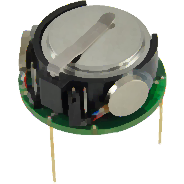
\includegraphics{kilogo.png}}
\author{Simon Lejoly}
\date{May 2021}

\begin{document}

\maketitle

\newpage

\tableofcontents

\newpage

\section{Overview of KiloGuide}

KiloGuide is a simple guide about \href{https://kilobotics.com}{kilobots}, small physical robots used in swarm robotics. The guide currently contains 2 sections of 5 tutorials, covering the most important aspects of kilobots. It explains how to perform various tasks such as calibration or code compilation and provides multiple small projects to illustrate how coding for kilobots is done.

This programmer guide describes how KiloGuide was implemented and how to bring modifications to it.

\section{Tools and references}

This section presents all the different tools that were used to implement KiloGuide.

\subsection{Markdown}

Markdown is a widespread markup language used to format text easily. It was chosen for being easy to write and to convert to other formats (html, pdf, ...) by applying custom styles.

\\\

References can be found \href{https://daringfireball.net/projects/markdown/}{here}.

\subsection{MKDocs and extensions}

\subsubsection{MKDocs}

MKDocs is a static site generator. It takes a config file and some markdown files and turns them into a fully-working html website, applying customizable styles in the process. It was chosen for its simplicity.

\\\

References can be found \href{https://www.mkdocs.org}{here}. 

\subsubsection{Extensions}

MKDocs enables the use of extensions for the markdown syntax. KiloGuide uses the "admonition" extension, providing syntax to create "note", "warning" and "error" boxes (among others).

\\\

References can be found \href{https://python-markdown.github.io/extensions/admonition/}{here}.

\subsection{ReadTheDocs}

ReadTheDocs is a well-known hosting website for open-source projects documentations. KiloGuide doesn't use ReadTheDocs to host its website, but it uses the very practical ReadTheDocs theme to style its pages. Plus, MKDocs supports the "ReadTheDocs" theme natively.

\\\

References can be found \href{https://readthedocs.org}{here}.

\subsection{GitHub and GitHub Pages}

\subsubsection{GitHub}

GitHub is a hosting platform built on the Git technology. It is used to host KiloGuide's source code and documentation. You can acces KiloGuide's repositry \href{https://github.com/SimLej18/KiloGuide}{here}.

\\\

References can be found \href{https://github.com/}{here}

\subsubsection{GitHub Pages}

GitHub Pages is the documentation hosting service of GitHub. It is used to host KiloGuide's website, \href{https://simlej18.github.io/KiloGuide/}{here}.

\\\

References can be found \href{https://pages.github.com}{here}

\section{Repository Structure}

This section describes the structure of KiloGuide's repository.

\begin{center}
    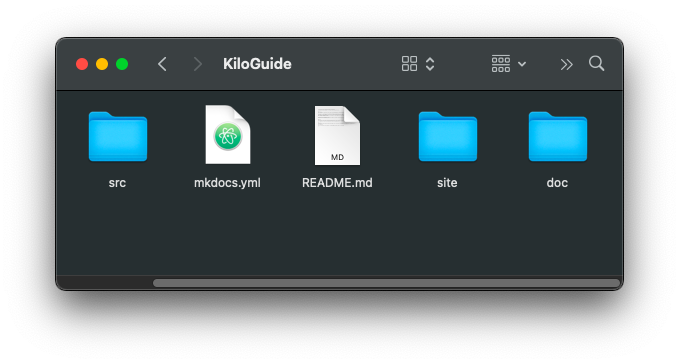
\includegraphics[scale=0.5]{structure.png}
\end{center}

\subsection{"README.md" file}

The "README" file contains a description of KiloGuide. It serves as a starting point to understand the purpose of KiloGuide and how it was built.

\subsection{"mkdocs.yml" file}

"mkdocs.yml" is the configuration file used by MKDocs to build KiloGuide. It specifies the name and structure of the website, the theme and extensions to use and various parameters.

\subsection{"src" directory}

The "src" directory contains the true body of KiloGuide. There you will find the various markdown files, each representing a specific page of KiloGuide. The "src" directory has the same structure as KiloGuide : the "home" and "about" pages are at its root and the various tutorials and guides are dispatched in their respective directories. You will also find the "to-be-implemented.md" file, which can be used while implementing some parts of the guide.

The "src" directory also contains "resources", a directory containing the images used in KiloGuide and the source code of all tutorials for them to be downloaded.

\subsection{"site" directory}

The "site" directory is automatically built by MKDocs after using the "mkdocs build" command. It contains the generated html static files, including the "index.html" file, the starting point of the guide. This directory is not available directly in the "main" branch of the GitHub repository, but its content is copied in the "gh-pages" branch to make the website available online via GitHub Pages.

\subsection{"doc" directory}

The "doc" directory contains the documentation of KiloGuide : its User Guide and its Programmer Guide. Each document is available in an editable ".tex" format as well as a shareable ".pdf" format.

\newpage

\section{Add a new page}

In this section, we cover the process of publishing a new page to KiloGuide step by step. This method should also make you understand how you can modify or delete existing pages.

\subsection{Write the page}

The first step is obviously to write the new page in markdown. You can find references on how to write your pages \href{https://www.mkdocs.org/user-guide/writing-your-docs/#writing-with-markdown}{here}. Here is an example of a new page:

\begin{center}
    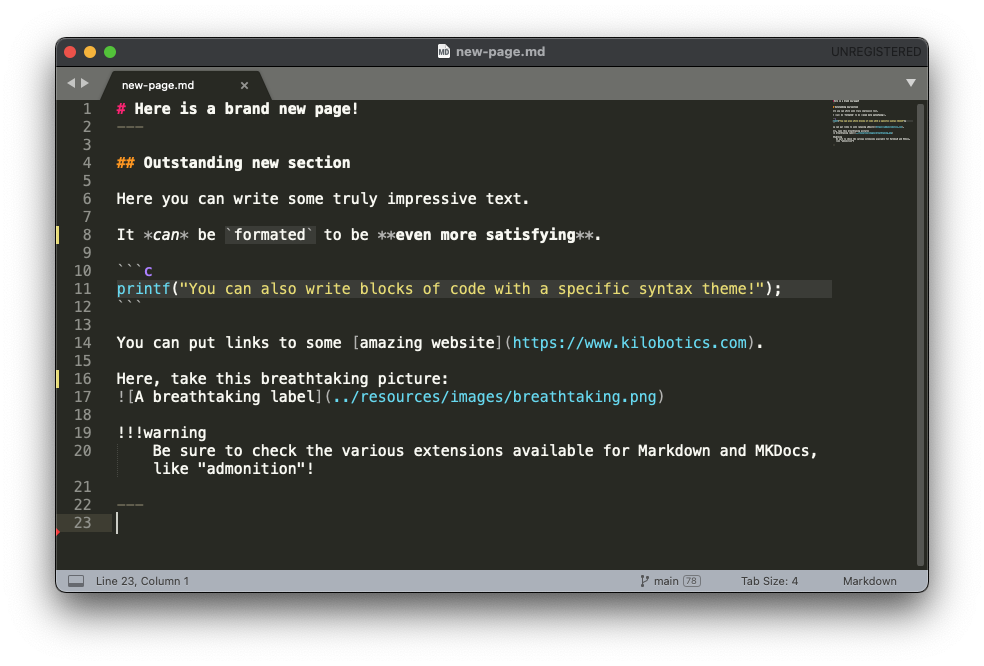
\includegraphics[scale=0.45]{new-page-md.png}
\end{center}

\subsection{Add the page to the guide}

Now, you need to tell MKDocs what to do with your file. This is done using the "mkdocs.yml" file, where you can link markdown files in your project to where they will be displayed in the website:

\begin{center}
    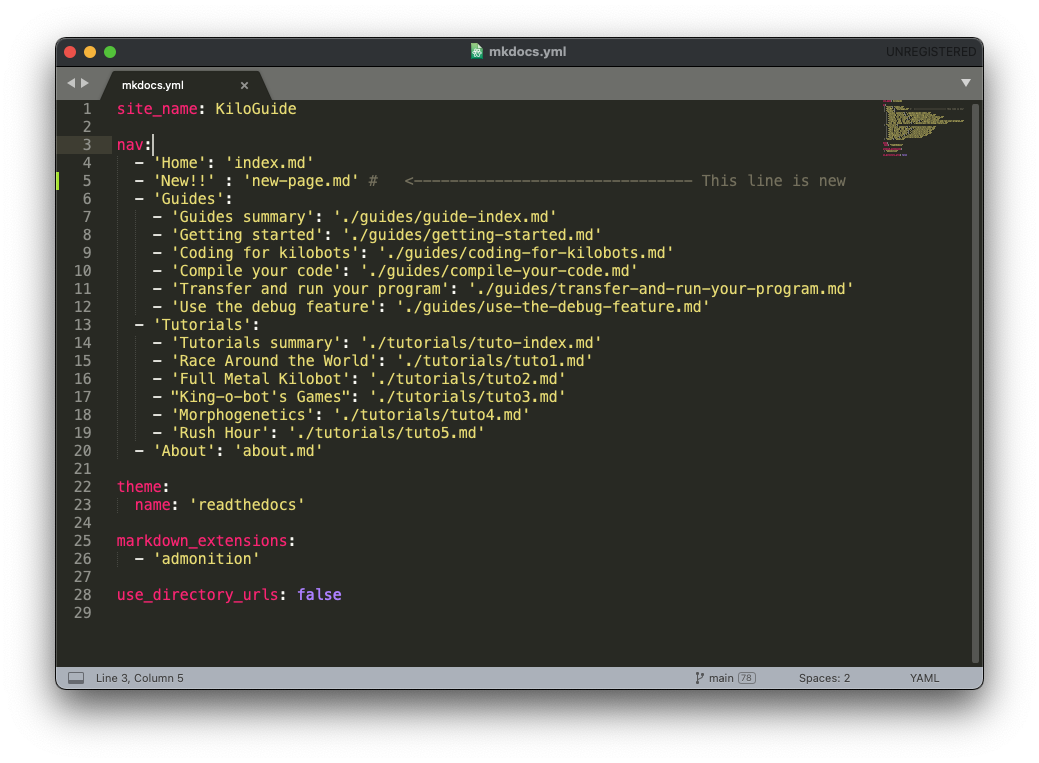
\includegraphics[scale=0.4]{new-config.png}
\end{center}

\subsection{See your new page}

You probably want to see what your new page looks like by now. This can be done by opening a terminal, navigating to the root of your MKDocs project and executing the command "mkdocs serve". If everything went right, you should now be able to access KiloGuide at your localhost address : \href{http://127.0.0.1:8000}{http://127.0.0.1:8000}. You should see that a new page popped in the menu bar! Click on it and there it is:

\begin{center}
    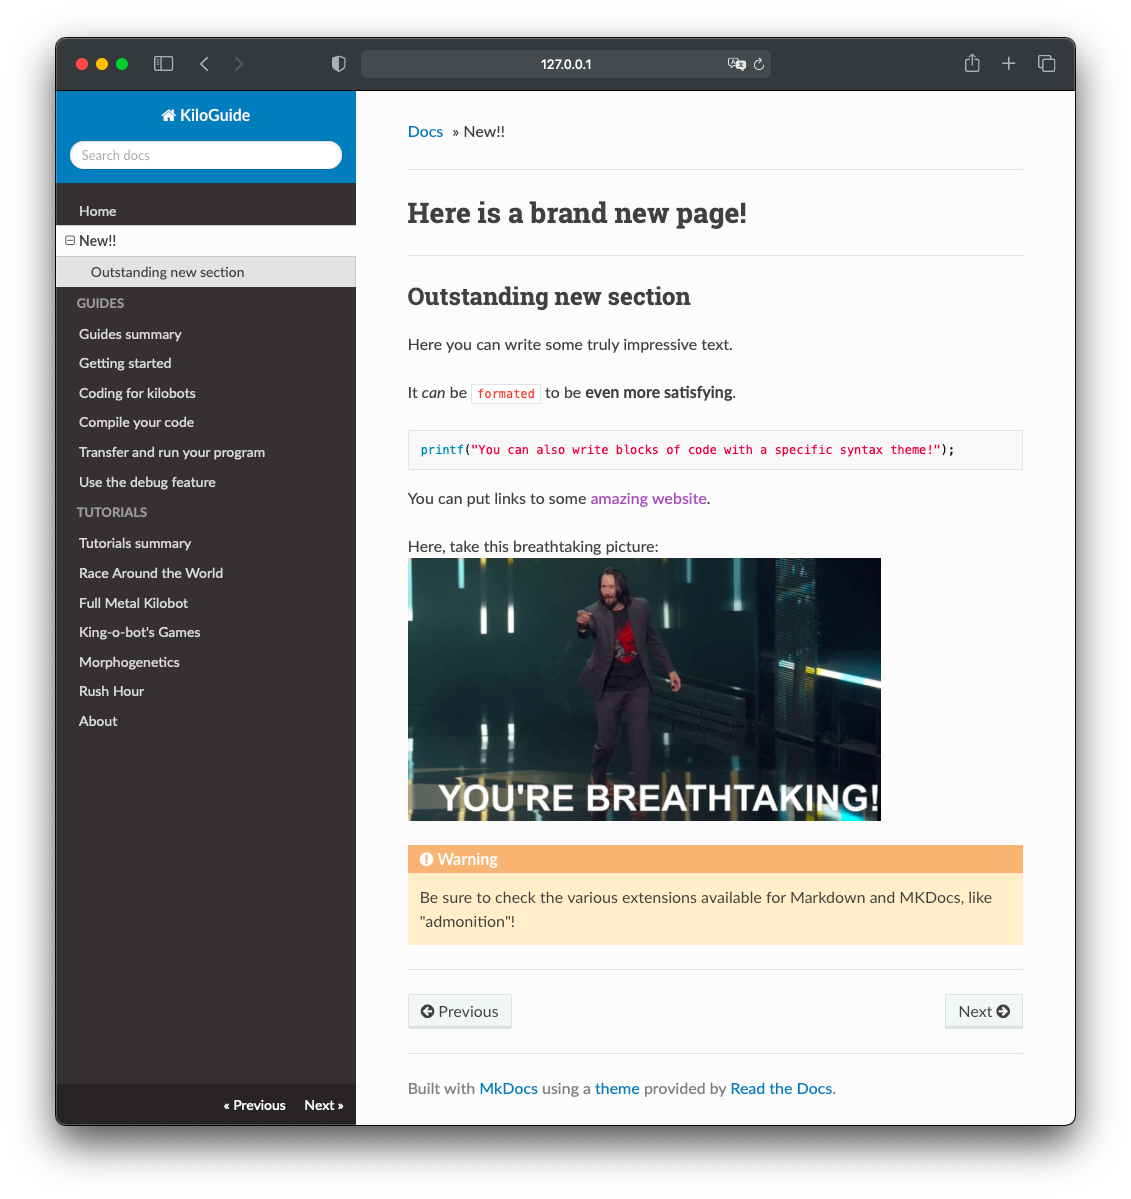
\includegraphics[scale=0.4]{new-page.png}
\end{center}

\subsection{Publish the new version to GitHub Pages}

To publish the new version of KiloGuide, you first need to build it. This can be done by executing the command "mkdocs build" at the root of your mkdocs project. After executing the command, the "site" directory should be created or updated. It should look something like this:

\begin{center}
    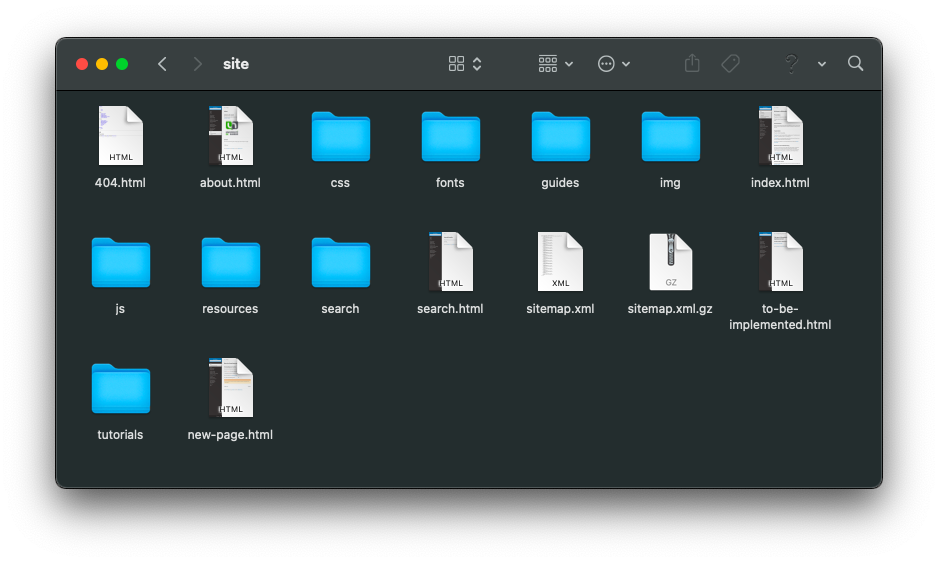
\includegraphics[scale=0.4]{new-site.png}
\end{center}

To make KiloGuide accessible through GitHub Pages, you need to push the content of "site" to the branch "gh-pages" of KiloGuide's repository. You will find reference regarding this process \href{https://www.mkdocs.org/user-guide/deploying-your-docs/#github-pages}{here}.

\section{Edit the documentation}

The documentation of KiloGuide is composed of its User Guide and the Programmer Guide you are currently reading. Both documents were written using LaTeX. They can be found in the 'doc' directory of KiloGuide's repository. You can  edit them using the TeX editor of your choice.

\section{Contact}

KiloGuide and its  programmer guide were written by \emph{Simon Lejoly} (\href{mailto:simonlejoly@icloud.com}{simonlejoly@icloud.com}) and are part of a project conducted by the \emph{University of Namur}.

\\\

Some of the content of this programmer guide, including images, may be subject to copyright.\\\\

\begin{center}

\includegraphics[scale=0.23]{unamur.png}
\end{center}

\end{document}
